\chapter{Fundamentals}

\section{What is a graph?}%
\label{sec:1.1whatisagraph}

A graph is a pair consisting of vertices and edges. It is usually denoted $G = (V,E)$.

\begin{figure}[ht]
	\centering
	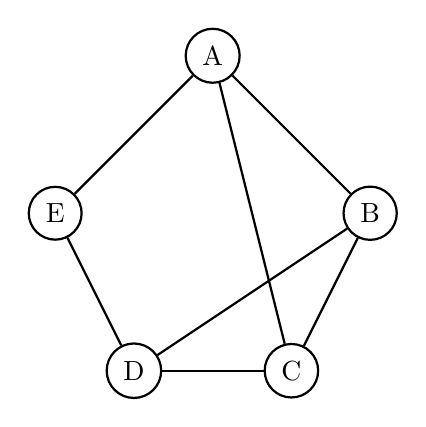
\begin{tikzpicture}[node distance={30mm}, thick, main/.style = {draw, circle}]

		\node[main] (A) at (0,0) {A};
		\node[main] (B) at (2,-2) {B};
		\node[main] (C) at (1,-4) {C};
		\node[main] (D) at (-1,-4) {D};
		\node[main] (E) at (-2,-2) {E};

		\draw (A) -- (B);
		\draw (B) -- (C);
		\draw (C) -- (D);
		\draw (D) -- (E);
		\draw (E) -- (A);
		\draw (A) -- (C);
		\draw (B) -- (D);
	\end{tikzpicture}
	\caption{\label{fig:graph1} A graph $G = (V,E)$}
\end{figure}

The graph seen in Figure~\ref{fig:graph1} features set of vertices $V = \{A, B, C, D, E\}$ and edges $E = \{AB, BC, CD, DE, EA, BD, AC\}$.

We say that an edge has \textit{endpoints}, which it \textit{connects}. Therefore, the edge $AB$ has endpoints $A$ and $B$.

It is important to remember that the visual representation seen of the graph in Figure~\ref{fig:graph1} is only a representation. The graph itself is just the set of vertices and edges connecting the vertices. Therefore, the graph can be represented in many ways, even graphically.

An edge can also be a \textbf{loop}. A loop is an edge that goes from a vertex and goes back to the same vertex without having any vertices in between. An example can be seen in Figure~\ref{fig:loop}.

\begin{figure}[ht]
	\centering
	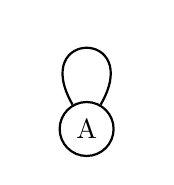
\begin{tikzpicture}[node distance={30mm}, thick, main/.style = {draw, circle}]

		\node[main] (A) at (0,0) {A};

		\draw (A) to[out=60, in=120, looseness=8] (A);
	\end{tikzpicture}
	\caption{\label{fig:loop} A loop.}
\end{figure}

Furthermore, a graph can contain \textbf{multiple edges} (also called \textbf{parallel edges}). This allows to edges to have the same pair of endpoints. And example of this can be seen in Figure~\ref{fig:parallel-edges}.

\begin{figure}[ht]
	\centering
	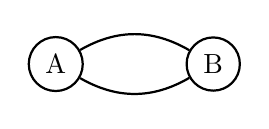
\begin{tikzpicture}[node distance={30mm}, thick, main/.style = {draw, circle}]

		\node[main] (A) at (0,0) {A};
		\node[main] (B) at (2,0) {B};

		\draw (A) to[bend left] (B);
		\draw (A) to[bend right] (B);
	\end{tikzpicture}
	\caption{\label{fig:parallel-edges} Parallel Edges.}
\end{figure}

\begin{definition}[Simple Graph]
	A \textbf{simple graph} is a graph without loops or parallel edges. Thus $\forall e \in E(G)$ $e$ is unique, and its endpoints cannot be the same.
\end{definition}

Two vertices connected by an edge are said to be \textbf{adjacent}. Given two adjacent vertices $A$ and $B$ this can be written $A \leftrightarrow B$. Additionally, we say that $A$ is a neighbour of $B$, and $B$ is a neighbour of $A$. The edge $AB$ is \textit{incident} to the vertex $A$ and $B$.

To introduce the concept of \textit{complement graphs} we will come up with an example of modeling graphs.

\begin{example}
	Consider six people, $a, b, c, d, e, f$. Amongst these people, each two persons are either friends, or strangers. We can turn this into a graph, calling it the friendship-graph. For each person $a$ we have a vertex, and for each friendship, we have an edge between the vertices.


	\begin{center}

		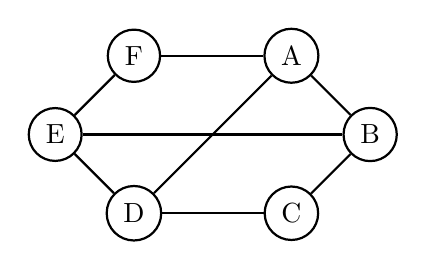
\begin{tikzpicture}[node distance={30mm}, thick, main/.style = {draw, circle}]

			\node[main] (F) at (-1,0) {F};
			\node[main] (A) at (1,0) {A};
			\node[main] (B) at (2,-1) {B};
			\node[main] (C) at (1,-2) {C};
			\node[main] (D) at (-1,-2) {D};
			\node[main] (E) at (-2,-1) {E};

			\draw (A) -- (B);
			\draw (B) -- (C);
			\draw (C) -- (D);
			\draw (D) -- (E);
			\draw (E) -- (F);
			\draw (F) -- (A);
			\draw (E) -- (B);
			\draw (D) -- (A);
		\end{tikzpicture}
	\end{center}

	This graph shows the friendships between the six people. However, it also implicitly shows how many are strangers, namely those who do not have an edge between them. If we turn this into a graph, where there is an edge between all those vertices where there was not an edge before, we get the \textit{complement}  of this graph, written $\overline{G}$.
	\begin{center}

		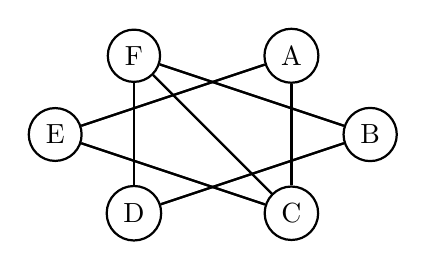
\begin{tikzpicture}[node distance={30mm}, thick, main/.style = {draw, circle}]

			\node[main] (F) at (-1,0) {F};
			\node[main] (A) at (1,0) {A};
			\node[main] (B) at (2,-1) {B};
			\node[main] (C) at (1,-2) {C};
			\node[main] (D) at (-1,-2) {D};
			\node[main] (E) at (-2,-1) {E};

			\draw (F) -- (B);
			\draw (F) -- (C);
			\draw (F) -- (D);
			\draw (A) -- (E);
			\draw (A) -- (C);
			\draw (B) -- (F);
			\draw (B) -- (D);
			\draw (C) -- (A);
			\draw (C) -- (F);
			\draw (C) -- (E);
			\draw (D) -- (F);
			\draw (D) -- (B);
			\draw (E) -- (A);
			\draw (E) -- (C);
		\end{tikzpicture}
	\end{center}

	Thus we can make the connection that $e \in E(G) \iff e \notin E(\overline{G})$.
\end{example}

A \textbf{clique} in a graph $G$ is a set of pairwise adjacent vertices.

\begin{figure}[ht]
	\centering
	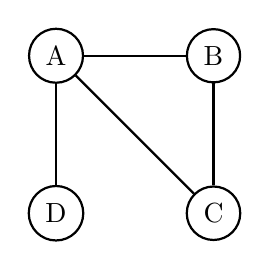
\begin{tikzpicture}[node distance={30mm}, thick, main/.style = {draw, circle}]

		\node[main] (A) at (0,0) {A};
		\node[main] (B) at (2,0) {B};
		\node[main] (C) at (2,-2) {C};
		\node[main] (D) at (0,-2) {D};

		\draw (A) to (B);
		\draw (B) to (C);
		\draw (C) to (A);
		\draw (D) to (A);
	\end{tikzpicture}
	\caption{\label{fig:clique} A graph with a clique $\{A, B, C\}$.}
\end{figure}

In Figure~\ref{fig:clique} is a representation of a graph with a clique $\{A, B, C\}$. The $D$ however, is not part of the graph, as it is not connected to all other vertices.

On the other end is the \textbf{independent} (or \textbf{stable}) set, which is a set of pairwise nonadjacent vertices. In Figure~\ref{fig:clique} an example as $\{D, C\}$ as they have no edges in common.


A \textbf{bipartite} graph is a graph which can be partitioned into two (possibly empty) disjoint independent sets.


\begin{figure}[ht]
	\centering
	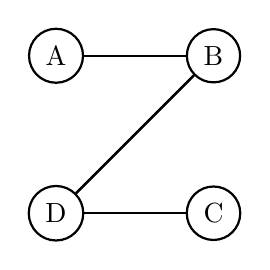
\begin{tikzpicture}[node distance={30mm}, thick, main/.style = {draw, circle}]

		\node[main] (A) at (0,0) {A};
		\node[main] (B) at (2,0) {B};
		\node[main] (C) at (2,-2) {C};
		\node[main] (D) at (0,-2) {D};

		\draw (A) to (B);
		\draw (B) to (D);
		\draw (D) to (B);
		\draw (C) to (D);
	\end{tikzpicture}
	\caption{\label{fig:bipartite} A bipartite graph.}
\end{figure}

In Figure~\ref{fig:bipartite} we see a graph which can be partitioned into two sets $X = \{A, D\}$ and $Y = \{B, C\}$ who have no edges in common. We can generalize this to be more than two partitions, in that case we call it a $k$-partite graph.

With the notion of $k$-partite graphs we can introduce the concept of \textbf{graph colouring}. Given a graph $G = (V,E)$, how many colors do we need, such that each vertex has a different color than its neighbours? For a bipartite graph, the answer is 2. In general, for a $k$-partite graph, the answer is $k$.


Moving on to the notion of \textit{paths} and \textit{cycles}. A \textbf{path} is a sequence of distinct adjacent vertices. A \textbf{cycle} is identical to a path, except it must begin and end with the same vertex. Examples can be seen in Figures~\ref{fig:cycle} and~\ref{fig:path}.

\begin{figure}[ht]
	\centering
	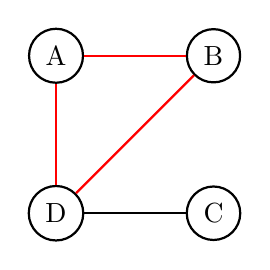
\begin{tikzpicture}[node distance={30mm}, thick, main/.style = {draw, circle}]

		\node[main] (A) at (0,0) {A};
		\node[main] (B) at (2,0) {B};
		\node[main] (C) at (2,-2) {C};
		\node[main] (D) at (0,-2) {D};

		\draw[red] (A) to (B);
		\draw[red] (B) to (D);
		\draw[red] (D) to (A);
		\draw (C) to (D);
	\end{tikzpicture}
	\caption{\label{fig:cycle} A cycle $\{A, B, D\}$.}
\end{figure}
\begin{figure}[ht]
	\centering
	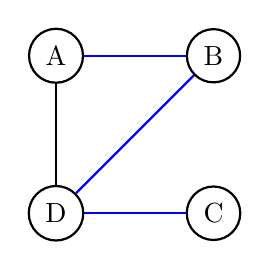
\begin{tikzpicture}[node distance={30mm}, thick, main/.style = {draw, circle}]

		\node[main] (A) at (0,0) {A};
		\node[main] (B) at (2,0) {B};
		\node[main] (C) at (2,-2) {C};
		\node[main] (D) at (0,-2) {D};

		\draw[blue] (A) to (B);
		\draw[blue] (B) to (D);
		\draw (D) to (A);
		\draw[blue] (C) to (D);
	\end{tikzpicture}
	\caption{\label{fig:path} A path $\{A, B, D, C\}$.}
\end{figure}

A \textbf{subgraph} is part of another graph. We say that $H$ is a subgraph of $G$ if $V(H) \subseteq V(G)$ and $E(H) \subseteq E(G)$. Furthermore, we say that $G$ \textbf{contains} $H$. As paths and cycles are both subgraphs, we can say that a graph $G$ can \textit{contain} a specific path or cycle.

So far we have only looked at visual representations of graphs in the form of circles as vertices and lines as edges. You can also represent graphs as matrices. Given a graph $G = (V,E)$ where $V = \{A, B, C, D\}$ and $E = \{E_{1}, E_{2}, E_{3}, E_{4}, E_{5}\}$ where $E_{1} = ab, E_{2} = bc, E_{3} = bc, E_{4} = ac$ and $E_{5} = cd$ we can represent these as an \textit{Adjacency Matrix} and an \textit{Incidence Matrix}. An adjacency matrix is a matrix where $A_{i,j}$ contains the number of edges between $i$ and $j$. This also means that the adjacency matrix is symmetric. In the \textit{incidence matrix} $M_{i,j}$ contains a $1$ if $j$ is an edge which is incident to $j$. This means that the incidence matrix' size is determined by the number of edges \textit{and} vertices, while the adjacency matrix' size is determined solely by the number of vertices.

% First matrix (Adjacency Matrix)
The adjacency matrix:
\[
	\begin{array}{c|cccc}
		  & a & b & c & d \\
		\hline
		a & 0 & 1 & 1 & 0 \\
		b & 1 & 0 & 2 & 0 \\
		c & 1 & 2 & 0 & 1 \\
		d & 0 & 0 & 1 & 0 \\
	\end{array}
\]

\hspace{1cm} % Horizontal space between the two matrices

The incidence matrix:
% Second matrix (Incidence Matrix)
\[
	\begin{array}{c|ccccc}
		  & e_1 & e_2 & e_3 & e_4 & e_5 \\
		\hline
		a & 1   & 0   & 0   & 1   & 0   \\
		b & 1   & 1   & 1   & 0   & 0   \\
		c & 0   & 1   & 1   & 1   & 1   \\
		d & 0   & 0   & 0   & 0   & 1   \\
	\end{array}
\]

Now we turn to the question of \textbf{isomorphism}. Given two graphs $G$ and $H$, is there a function $f : V(G) \rightarrow V(H)$ that maps such that $uv \in E(G) \iff f(u)f(v) \in  E(H)$. If such a function exists, we say that $G$ is \textbf{isomorphic} to $H$. We write this $G \cong H$.

We define the \textit{isomorphism class} to be an equivalence class of graphs under the isomorphism relation. I.e., all graphs that are isomorphic to each other form an isomorphism class.

Given a graph with $n$ vertices, how many graphs are possible? I.e., how many ways can we arrange the edges? Given a pair of vertices, there are two options: either an edge connects them, or there is no edge to connect them. Thus there are $2^{\binom{n}{2}}$ possible graphs on $n$ vertices. The question of how many isomorphism classes there are on $n$ vertices is not easy to answer.

Some other classes of graphs are:
\begin{itemize}
	\item $P_{n}$: A path with $n$ vertices.
	\item $C_{n}$: A cycle with $n$ vertices.
	\item $K_{n}$: A complete graph with $n$ vertices.
\end{itemize}
In a complete graph, all vertices are pairwise adjacent, meaning there is an edge between all vertices. We denote the complete graph $K_{n}$, and the \textbf{complete bipartite graph} $K_{r,s}$ where $r$ is the number of vertices in one set and $s$ the number of vertices in the other. Then for each $v \in R$, there is an edge to all $v \in S$, and the other way around. However, there is no edge between the vertices in respectively $R$ and $S$.

A special graph, the Petersen graph, is probably the most famous graph in all of graph theory. The graph is the result of  the following statement: $(ij)$ and $(kl)$ are adjacent if $\{i,j\} \cap \{k,l\} = \emptyset$.

A graph is said to be \textbf{self-complementary} if it is isomorphic to its complement. Some examples are $P_{4}$ and $C_{5}$.

The \textbf{decomposition} of a graph is a list of subgraphs such that every edge appears in exactly one subgraph in the list.

The \textbf{girth} of a graph is the length of its shortest cycle.

An automorphism of $G$ is an isomorphism from $G$ to itself. A graph is said to be \textbf{vertex-transitive} if for every pair $u, v \in V(G)$ there exists an automorphism that maps $u$ to $v$.

\section{Paths, Cycles and Trails}%
\label{sec:label}

As we have already talked about briefly, paths are sequences of vertices and edges $v_{0}e_{1}v_{1}\ldots e_{k}v_{k}$. Trails and paths are the same. However, we distinguish between these as such:
\begin{itemize}
	\item \textbf{Walk}: No constraints.
	\item \textbf{Trail}: All edges must be distinct.
	\item \textbf{Path}: All vertices must be distinct (and by extension edges).
\end{itemize}

We write $(u,v)$-(walk,path,trail) in order to specify a (walk,path,trail) which starts at vertex $u$ and ends at vertex $v$.

\begin{lemma}
	Every $(u,v)$-walk contains a $(u,v)$-path.
\end{lemma}

\begin{proof}
	We prove this by induction on the number of edges, $m$. The walk itself we call $W$.\\
	\noindent
	\textbf{Base Case $m = 0$}: $W$ is a $(u,v)$-path with 1 vertex.\\
	\noindent
	\textbf{Inductive Step}: Assume true for all smaller $m$.\\
	\noindent
	If no vertex in walk $W$ repeats, then $W$ is a $(u,v)$-path. If a vertex repeats, then we can write the walk as $v_{0}v_{1}v_{2} \cdots v_{i} \cdots v_{j}v_{j+1} \cdots v_{k}$ where the path has length $k$. In this case, there must be an $i$ and $j$ such that $v_{i} = v_{j}$. Thus, we can ignore the part between, $v_{i}v_{i+1} \cdots v_{j-2}v_{j-1}$, and have a resulting $(u,v)$-path.
\end{proof}

We say that a graph $G$ is connected, if $\forall u,v \in V(G)$ there is a $(u,v)$-path. The connected \textbf{components} of $G$ are the maximal connected components of $G$.

The \textbf{order} of the graph is the number of vertices. The \textbf{size} of the graph is the number of edges.
\begin{proposition}
	Every (simple) graph of order $n$ and size $k$ has at least $n-k$ components.
\end{proposition}
\begin{proof}
	We prove by induction on the number of edges $m$.\\
	\noindent
	\textbf{Base Case} $m = 0$: A graph with $n$ vertices and $0$ edges has $n - k = n - 0 = n$ components.\\
	\noindent
	\textbf{Inductive Step}: Assume for smaller $m$.\\
	\noindent
	Given a graph with $n$ vertices and $k$ edges, if we remove one edge, we can at most add one new component.
\end{proof}

A vertex $v \in V(G)$ is a \textit{cut-vertex} if deleting $v$ increases the number of components. Similarly, an edge $e \in E(G)$ is \textit{cut-edge} if deleting it increases the numbre of components.

\begin{theorem}
	An edge is a cut-edge if and only if it belongs to no cycle.
\end{theorem}
\begin{proof}
	$\Rightarrow$\\
	\noindent
	Assume that the edge is not a cut edge, if it belongs to no cycle. Thus, removing it would not create a new component. However, it would create a new component, as when there is no cycle it must be split into two. This is a contradiction.\\
	\noindent
	$\Leftarrow$\\
	\noindent
	TONCAS.
\end{proof}

\begin{theorem}[König 1936]
	A graph is bipartite if and only if it has no odd cycle.
\end{theorem}

\begin{proof}
	Let $G$ be a bipartite graph with partite sets $A$ and $B$.\\\\
	\noindent
	$\Rightarrow$\\
	\noindent
	Starting a walk in $A$, the walk will alternate between the partite sets $A$ and $B$ between each edge. Thus, when it returns it will have an even number of edges. Therefore, the cycle will be even.\\
	\noindent
	$\Leftarrow$\\
	\noindent
	We prove this for each component of $G$.
	Let $C$ be a component of $G$ and let $x \in V(C)$. For each $y \in V(C)$ let $f(y)$ be the distance from $x$ to $y$. This distance is the shortest distance, and thus the length of the shortest $(x,y)$-path.

	Let $X = \{u \mid f(u) \text{ is even}\}$ and $Y= \{u \mid f(u) \text{ is odd}\}$. We will show that $X$ and $Y$ are independent, and thus $C$ is bipartite.

	For the sake of contradiction, assume that there is an edge $v_{1}v_{2} \in E(C)$ in $Y$ (or $X$). There exists  a $(x,v_{i})$-path $P_{i}$ of length $f(v_{i})$ for $i = 1,2$. Let $z \in V(P_{1}) \cap V(P_2)$ be chosen such that $f(z)$ is maximum.

	Let $P_{i}'$ be the $(z,v_{i})$-subpath of $P_{i}$, for $i = 1,2$. $|E(P_{i}')| = f(v_{i}) - f(z)$ for $i = 1,2$.

	%% NÅET TIL s. 143 i Long, 45 i short.

\end{proof}

%%% Local Variables:
%%% mode: latex
%%% TeX-engine: luatex
%%% TeX-command-extra-options: "-shell-escape"
%%% TeX-master: "main"
%%% End:
